\documentclass{article}
\PassOptionsToPackage{numbers,sort&compress}{natbib}
\usepackage[dblblindworkshop]{neurips_2026}
\workshoptitle{AgenticOS}
\usepackage[utf8]{inputenc}
\usepackage[T1]{fontenc}
\usepackage{booktabs}
\usepackage{amsmath}
\usepackage{microtype}
\usepackage{xcolor}
\usepackage{hyperref}
\hypersetup{colorlinks=true,linkcolor=black,citecolor=black,urlcolor=black}
\usepackage{array}
\usepackage{pifont}
\usepackage{graphicx}
\newcommand{\cmark}{\ding{51}}
\newcommand{\xmark}{\ding{55}}
\title{What the Final Patch Hides:\\Event-Level Regression Measurement for Coding-Agent Harnesses}
\author{Anonymous Authors\\AgenticOS Workshop Submission}
\begin{document}
\maketitle
\begin{abstract}
Coding agents are graded on the final patch alone. We instrumented an unmodified coding agent to replay the benchmark's previously-passing tests after every edit, and found that transient regressions are common but almost never survive to the graded patch. Replacing our own harness's model-written check with an execution-grounded one recovers the resolve that check was destroying (13 to 26 of 40; exploratory, and circular by construction). The instrument commits the working tree after every mutating tool call and replays the benchmark's oracle at every commit inside its pinned container. We applied it to mini-swe-agent 2.4.6 unmodified, keeping its own loop, prompts, model layer, budgets, and submission protocol, and replacing only its environment object. On 40 SWE-bench Verified tasks it resolves 34 of 40 with \texttt{claude-sonnet-4-6} and 33 of 40 with \texttt{gpt-5.6-sol}, and every run ends with a changed tree. Eleven of the 80 broke previously-passing test functions, 135 counted per run and 100 distinct, one still failing when the official grader read the final tree. Its own testing does not close the gap. Over the window in which each test was broken, no test command ran the broken test in 6 of the 10 classifiable cases. In the other 4 one ran it and printed the failure by name. A method reading only the agent's logs is structurally blind to most of them. The undercount holds in our harness under rollback (146 test functions broken across 8 of 47 runs, one still failing) and on SWE-bench Live. Two caveats we make measurable: rollback leaves clean trees partly because 17 of its 37 runs ship a tree they never changed, and a model-stack difference on Verified does not survive a change of scaffold. The instrument has its own blind spot. Nine of the ten trees that killed the suite recorded no event. We will release the instrument, its validation protocol, and the archived timelines. Appendix A catalogues 28 measurement defects met while building it, 23 of which produced plausible numbers rather than errors.
\end{abstract}

\section{Introduction}

Benchmarks for coding agents grade the final patch. SWE-bench \cite{ref1} and its Verified subset \cite{ref2} apply the submitted patch and report whether the target tests pass and the previously passing ones still pass, and work on agent-caused regressions counts what the submitted patch breaks \cite{ref8}. That convention cannot see what happens while the agent works, because an agent that breaks a test at step three and repairs it at step five submits a clean patch. Two questions are left open: how often do agents break existing behaviour during a run, and how much survives?

The answer was smaller than we expected, and not in the place we expected. Agents break the oracle often and almost always repair it, so what the endpoint misses is transient and not shipped. We measure the timeline instead of the endpoint. Every mutating tool call becomes a commit on a git reference the agent cannot see, and the oracle is re-run at every commit inside the benchmark's pinned container. An agent operating system needs this observation primitive before it can build a recovery primitive. We contribute:

\begin{enumerate}
\item \textbf{An instrument for event-level regression measurement}, applicable to an agent we did not write. Every mutating tool call becomes a commit on a hidden git reference, and the benchmark's previously-passing oracle is replayed at every recorded state inside its pinned container (Section 3).
\item \textbf{The measurement on an unmodified public scaffold.} mini-swe-agent 2.4.6 keeps its own loop, prompts, model layer, budgets, and submission protocol. Only its environment object is ours. It resolves 34 and 33 of 40 under two model families and breaks 135 oracle test functions counted per run (100 distinct) across 11 of the 80 runs, one still failing at grade time. In 6 of the 10 classifiable cases its own test commands never ran the test it broke (Section 5.1).
\item \textbf{The same measurement across recovery policies.} The undercount holds in our harness and on SWE-bench Live. But nearly half the rollback arm's runs ship a tree they never changed, so a clean final tree partly means no edits at all (Sections 5.2, 5.3, 5.5).
\item \textbf{Recovery policy depends on the monitor's precision.} With a model-written check, rollback buys 4 fewer contaminated trees for 11 fewer resolved instances (1 against 5; 13 against 24). Replacing that check with the repository's own oracle gets both: 26 resolved, no contaminated tree, and a lower cost per resolved instance than either. It is exploratory and circular by construction (Section 5.4).
\item \textbf{A catalogue of 28 measurement defects} found while building the instrument (Appendix A); 23 produced a plausible number rather than an error.
\end{enumerate}

All measurements are exploratory, on development slices excluded from future confirmatory study.

\section{Background and related work}

\textbf{Benchmarks and their validity.} SWE-bench \cite{ref1} grades a patch by tests that must go from failing to passing and tests that must keep passing. Verified \cite{ref2} is the human-screened subset, deprecated as a capability metric \cite{ref45}. Concerns about it have accumulated. They include contamination and memorisation \cite{ref6}, plausible-but-wrong patches overstating resolve by 6.2 points \cite{ref36}, and insufficient tests, which UTBoost \cite{ref7} augmented to expose mislabelled patches affecting 24.4\% of leaderboard entries. Rolling \cite{ref3,ref5}, private \cite{ref4}, and long-horizon \cite{ref23} alternatives came in response. TDAD \cite{ref8} measured regressions in \emph{submitted} patches on Verified (6.1\% of previously-passing tests, 30.2\% of non-empty patches) and reduced them with an impact-analysis map. Process-level benchmarks score intermediate states from logs \cite{ref34,ref35}, and AgentLens \cite{ref37} names regression cycles in 10.7\% of passing OpenHands runs, against our 11 of the 38 runs that edited substantially (29\%). A log-derived rate is bounded below by what the agent chose to run, and in 6 of our 10 classifiable cases it ran nothing that would have executed the broken test. We execute the oracle at every mutating call instead.

\textbf{Agent scaffolds and recovery.} SWE-agent \cite{ref9}, OpenHands \cite{ref10}, Agentless \cite{ref11}, and mini-swe-agent \cite{ref12} span the scaffold design space \cite{ref13,ref14}. Within-episode recovery appears as self-reflection \cite{ref15,ref16}, progress-gated recovery \cite{ref17}, checkpoint repair \cite{ref18}, and aligned checkpoints \cite{ref40}. Provenance-based recovery is surveyed in \cite{ref19}. Closest to us, Kim et al. \cite{ref38} match logged edits against the gold diff and recover agents that reach a gold-identical patch and then destroy it. Gao et al. \cite{ref39} bind verifier evidence to code states. Neither counts regressions or compares policies. Running the repository's tests during a run is deployed practice \cite{ref42,ref43}. Operating-system framings \cite{ref20} and the branch-context primitive \cite{ref41} supply scheduling and fork, commit, and abort, but do not observe the tree between actions. The regression problem is program repair's plausible-versus-correct patch problem \cite{ref26,ref28,ref29}, where regression tests are the main defence against overfitting \cite{ref27}. Trajectory-level evaluation \cite{ref21,ref22} argues resolve rate alone is uninformative. Public leaderboard trajectories record actions but not the tree at each step, which the instrument commits.

\section{Instrument}

\begin{figure}[t]\centering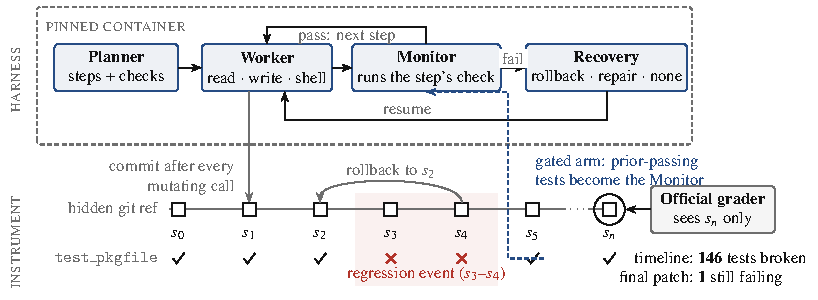
\includegraphics[width=0.46\linewidth]{fig_system.pdf}\caption{The harness and the instrument. Every mutating tool call commits the tree to a hidden git reference. After the run, the instance's previously-passing tests are replayed at every state. The test row shows one regressing at s$_3$--s$_4$ and repaired by a rollback to s$_2$, which the official grader, reading only s$_n$, never sees. The counts are the GPT-5.6 rollback arm's, over all 47 of its runs. In the gated arm (dashed), the timeline's tests serve as the monitor.}\label{fig:fig-system}\end{figure}

Figure~\ref{fig:fig-system} shows the harness and the instrument. \textbf{Observational timeline.} After every mutating tool call the working tree is committed to a git reference outside the agent's view (a private index keeps its own \texttt{git status} unchanged). Rollbacks and the run's end are observations too, and an archived run can be re-measured without re-running the agent. The agent's tools and the harness's checks execute inside the same pinned container as the replay, synchronised to the host tree the timeline records (Appendix A.2).

\textbf{Exhaustive replay.} For each observation the instance's previously-passing (PASS\_TO\_PASS) tests run inside the pinned container against that observation's tree. A regression event is a test that passes at one observation and fails at a later one. We replay every observation instead of bisecting, because a recovery policy makes verdicts non-monotone. Replay is scoped to the files holding those tests, which keeps it affordable on Verified (4 to 8 seconds per observation, about 26 CPU-minutes per sweep). Live's larger oracles cost tens of minutes per instance. Infrastructure failures during replay, and tests already failing in the unmodified image, are recorded as missing observations, not failures.

\textbf{Validation.} Five checks run before any paid experiment (negative and positive controls, the latter including \emph{recovered} regressions, a flake screen, an unknown-rate ceiling, a baseline liveness check), plus a golden check driving the gold patch through the agent's real tool path and a re-scoring control that re-measures an archived timeline with no model calls. Re-scoring four arms' bearing runs reproduced their episode counts and probe sets exactly. Appendix C gives the detail.

\section{Experimental setup}

\textbf{Benchmark and slice.} SWE-bench Verified is a measurement substrate here, not a leaderboard. Its pinned images and oracles make the measurement possible. A 40-instance development slice (16 from django), stratified and fixed before any measurement, was used throughout and is excluded from future confirmatory study. The GPT-5.6 stack also ran its first 10 as a calibration, and plain rollback ran twice. SWE-bench Live \cite{ref3}, built monthly from live repositories, is the second substrate, graded by its own harness whose rules we mirror. Its slice was fixed before any outcome (Appendix B) and its oracles are about twenty times larger (median 1,189 against 58 tests).

\textbf{Harness.} A planner decomposes the task into steps with verification commands, a worker executes each with three tools (read, write, shell), and a monitor runs the verification. On failure the recovery policy acts: \textbf{rollback} (reset to the last verified checkpoint and retry), \textbf{repair-in-place} (retry from the failed tree), or \textbf{no recovery} (the FAIL is final and the run ends). Runs have a \$4 work-cost cap. One instance under one policy is a cell. Each (stack, policy, substrate) triple is an arm.

\textbf{Public scaffold.} mini-swe-agent 2.4.6 \cite{ref12} runs unmodified (its own loop, prompts, model layer, 250-step and \$3 caps, and submission protocol) with only its environment object replaced, so every bash command executes in the benchmark's pinned container and the tree is committed to the hidden reference after each. The seam is inert but not invisible. The agent's \texttt{git diff} and \texttt{git status} show its own uncommitted edits and none of the instrument's commits, but the synthetic baseline carries a marker name 54 of the 80 runs saw, and we cannot settle here whether that changed behaviour. Six departures from its leaderboard configuration, a grid census putting its sampling inside our arms' range (a median of 3 and 2 tree-changing observations per run against our 2 to 5, at 9 to 15 bash commands each), and the rest are in Appendix C. We claim no equivalence to its published resolve rate, and because its budget differs in kind from our cap, no comparison between harnesses is tested.

\textbf{Models.} Two frontier stacks under identical harness, policy, instances and caps: \texttt{claude-opus-4-7}/\texttt{claude-sonnet-4-6} and \texttt{gpt-5.6-sol}/\texttt{gpt-5.6-terra} (planner/worker).

\textbf{Outcomes.} Resolve is the official grader's verdict on the final patch. Events are reported at three levels because a few runs produce most: incidents (observations at which at least one oracle test broke, the co-primary endpoint), declared events (one per test function and onset, parametrised variants collapsed), and bearing runs (runs with at least one event). Incident \emph{exposure} is a run's incident count. An event and a final-state failure are different objects, so the undercount is in matched units (test functions broken during a run against those still failing at the end). Contamination counts oracle tests failing in the graded patch, net of baseline-dead. A tree that kills the suite is graded as failing every test but is a missing observation for event counting, so a contaminated cell need not be a bearing run.

\textbf{Pre-declaration.} The event unit, the proceed criteria, and the recovery-policy contrast were declared before the relevant data existed, and the analysis was committed before either comparison arm finished. One amendment preceded unblinding and one grading correction followed it (Section 5.3, Appendix B).

\section{Results}

\subsection{An unmodified public scaffold breaks tests and puts them back}

mini-swe-agent 2.4.6 ran unmodified on the same 40 instances. With \texttt{claude-sonnet-4-6}, 34 of 40 resolved (35 rot-aware) over 2,101 bash commands for \$31.38. Four runs hit its own \$3 cap. Three of those still grade resolved, because resolve reads the final tree, not the patch the scaffold never submitted. With \texttt{gpt-5.6-sol}, 33 of 40 resolved (34) over 937 commands for \$12.13. None of the 80 ended byte-identical to its start.

The timeline recorded 56 events in 5 of the 40 Claude runs and 79 in 6 of the 40 GPT-5.6 runs, on 8 instances, 3 bearing under both. Those 11 runs broke 135 oracle test functions counted per run (100 distinct, because the stacks overlap on the three shared instances), and when the grader read the final tree exactly one was still failing, \texttt{test\_pkgfile} in pytest-6197 (Claude 0 of 56, GPT-5.6 1 of 79). The scaffold has no monitor or rollback, so every closure is an ordinary forward edit. The eleven stayed open for 1 to 22 bash commands (median 4), and three runs supply 81\% of the 135. Against exposure rather than attempts the rate is higher. No run making two or fewer tree-changing observations was bearing, and 11 of the 38 that made more broke something (29\%). Much of what the endpoint misses is a transient inside one logical edit, but transients are not free: 14\% of what these runs cost (\$1.29 of \$9.52) was spent while a regression was open.

\textbf{One run in full.} On django-12965 the GPT-5.6 scaffold read \texttt{SQLDeleteCompiler} for twelve commands, then at command 13 changed \texttt{single\_alias} to count active aliases with \texttt{<= 1}. Its own reproduction script crashed, and at command 15 \texttt{runtests.py delete} printed \texttt{ERROR: test\_fast\_delete\_large\_batch}. Command 16 replaced the edit, command 18 ran the suite clean, and the run graded resolved at 52 of 52. The timeline holds all of this. The graded patch holds none of it.

\textbf{Would its own testing have caught it?} For each breaking edit we read the trajectory over the window the test was broken, from the breaking command to just before the repair, asking whether a test runner ran, whether any run would have executed \emph{this} test, and whether its output showed the failure. Coverage is three-valued, with \emph{unknown} for runs that stopped early or were truncated (Appendix C). In 6 of the 10 classifiable cases the agent's own test commands never ran the broken test. In the other 4 they ran it and printed the failure by name, and it was repaired anyway. The eleventh is unknown, a \texttt{pytest -x} run that stopped earlier. Self-testing is blind to the first group and ignored on the second. The endpoint sees neither. With eleven cases this is a case series, not a rate.

\subsection{The same undercount in our harness}

\begin{figure}[t]\centering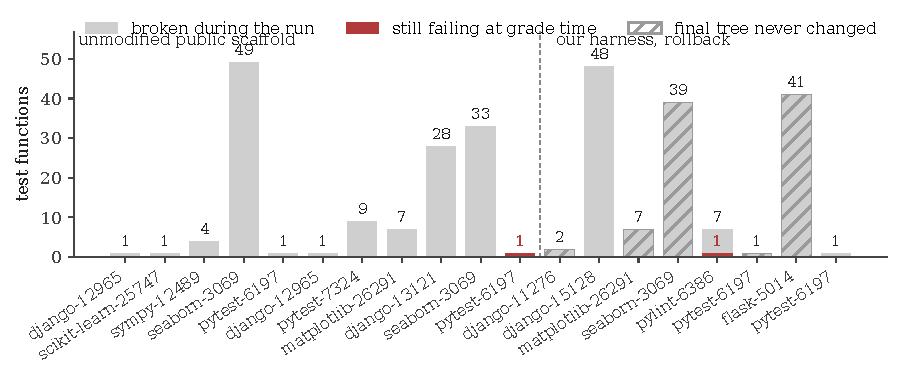
\includegraphics[width=0.66\linewidth]{fig_undercount.pdf}\caption{Every run that broke an oracle test, in matched units. Test functions broken on the timeline, dark where still failing at grade time. Left, the unmodified public scaffold under both models. Right, our rollback arm, hatched where the final tree is byte-identical to its start.}\label{fig:fig-undercount}\end{figure}

Under rollback the Claude stack resolved 13 of 40 (32.5\%, exact 95\% CI 18.6\% to 49.1\%) for \$34.24 and the GPT-5.6 stack 13 of 40 for \$8.14. A circuit breaker stopped three cells and a synchronisation defect lost two, so 37 were attempted and 35 graded (13 of 35, 37.1\%). Rates are out of 40 unless stated, and one instance is unresolvable under the current parser (Appendix A.3), putting the ceiling at 39 for every arm, the scaffold included. The median rollback run makes 4 mutating tool calls under GPT-5.6 and 3 under Claude.

Eight of the 47 GPT-5.6 rollback runs (the sweep and a 10-instance calibration) broke a previously-passing test, 146 test functions counting each run separately (145 distinct). One of those, \texttt{test\_can\_read\_toml\_env\_variable} in pylint-6386, was still failing at grade time. Three storms supply 88\% of the 184 declared events over all 47 runs. Table~\ref{tab:every-arm-on-both-substr}'s 140 is the sweep alone, and declared events are exposure only. Figure~\ref{fig:fig-undercount} shows every bearing run on both sides.

A clean tree does not always represent work. Excluding the hidden reference, 17 of the 37 rollback runs end byte-identical to their start, as do 19 of the Claude stack's 40, 4 under the gate, and 0 under repair-in-place. Four of the six bearing sweep runs shipped nothing. Over the two that delivered a patch, 1 of 55 broken test functions is still failing, so the claim rests on the public-scaffold arm, where no run ends unchanged.

Event frequency also differed by model stack, but does not generalise. Under the same harness and policy the Claude stack produced no events in 40 runs against the GPT-5.6 stack's 140 in 6 of 37 (one-sided Fisher p = 0.010; reassign three bearing runs and p = 0.11), yet the same \texttt{claude-sonnet-4-6} worker under unmodified mini-swe-agent is bearing on 5 of 40 with 56 events, and the difference is absent on Live. Model and adapter are confounded, and controls are in Appendix C.

A break that stops the suite from being collected opens no timeline event, because a test the parser never mentions counts as a missing observation, not a failure, while official grading scores such a patch as failing everything. Nine of the ten suite-killed trees across all arms recorded no event, so the two instruments miss different things.

\subsection{Recovery policy: what the clean final tree costs}

On the primary endpoint, contamination paired by instance, no recovery was worse than rollback on 9 instances and better on 1 (exact sign test p = 0.021). Repair-in-place was worse on 5, better on 1 (p = 0.22). Incident exposure, the co-primary, did not differ (p = 0.45 and 1.0). The arms cannot show the policy caused the difference. No recovery ends at the monitor's first FAIL, so its regressions arrive on the last tree-changing observation with nothing after them, and its 19-of-19 persistence is the stopping rule as much as the policy.

Rollback pays for its clean tree in delivered work, resolving 13 of 40 against 24 and 22, losing nine discordant pairs to repair-in-place and winning one (McNemar p = 0.021). The loss is the monitor's. Of the 18 failed rollback runs, 15 failed at the first step, and 9 of those instances were resolved by an arm that kept work the check rejected and the grader accepted, and 17 of 37 runs ended unchanged.

\textbf{Disclosure.} The first unblinding gave p = 0.375, because seven cells whose final trees killed the suite had been dropped as ungradable. Correcting the grader and re-grading those archived trees gives the 0.021 above, a rule change made after the data were seen (Appendix B).

\subsection{Replacing the check removes the tradeoff}

A fourth arm, added after unblinding (exploratory), replaces the planner-written check with the repository's own oracle, run after every attempt. A step is rejected only if a test that passed at the start now fails. It resolved \textbf{26 of 40 (65.0\%)}, above rollback's 13 and the ungated arms' 24 and 22, below the 34 and 33 mini-swe-agent reaches under a budget differing in kind (Table~\ref{tab:every-arm-on-both-substr}), with \textbf{no contaminated final tree} and 4 empty patches against rollback's 17. The guarantee is cheap. The gate runs at least 4 times in the median run at 4 to 8 seconds each, so 16 to 32 seconds of wall-clock and \$2.37 more model spend than rollback, and per resolved instance it costs \$0.40 against rollback's \$0.63 and repair-in-place's \$0.61. It beat rollback on 35 shared instances, winning 10 discordant pairs and losing 1 (p = 0.012), and repair-in-place 26 to 24 with 0 contaminated trees against that arm's 5. The gate gives a guarantee, not a rate, and it is circular. Its tests are the benchmark's own oracle (median ratio 1.00), so a clean tree follows whenever the gate saw the final tree and the grader reads what the gate read. A fifth arm weakens that, reading a deterministic half of the ids (2,278) and never the other half (2,585), on which the grader also rules \cite{ref44}. The split is over ids, not files, so a break reaching a held-out id usually reaches a watched one, and the held-out half bounds the leak instead of sampling it. A file-level or non-oracle gate would settle it. It resolved \textbf{28 of 40 (70.0\%)}, indistinguishable from the full gate (p = 0.73) and better than rollback (13 to 2, p = 0.007), with no held-out failure apart from the parser-capped instance.

\subsection{Replication on SWE-bench Live}

\begin{table}[t]\caption{Every arm on both substrates. \textbf{empty}: runs ending byte-identical to their start. \textbf{events}: declared (test function, onset) pairs, exposure only, never a denominator. \textbf{broken $\rightarrow$ left}: oracle tests broken during the bearing runs against those still failing at grade time. \textbf{inc.}: incidents, the pre-declared co-primary. \textbf{contam.}: graded cells failing an oracle test, net of baseline-dead. The Claude rollback arm's 1 is baseline rot, not agent damage (Appendix C). The public-scaffold rows ran under mini-swe-agent's own budget, not our cap. Composition and provenance: Appendix C.}\label{tab:every-arm-on-both-substr}
\centering\scriptsize\setlength{\aboverulesep}{0pt}\setlength{\belowrulesep}{0pt}\renewcommand{\arraystretch}{0.86}\setlength{\tabcolsep}{4pt}\begin{tabular}{llllllllll}
\toprule
substrate & arm & resolved & empty & events & inc. & bearing & broken $\rightarrow$ left & contam. & spend \\
\midrule
Verified & mini-swe-agent, Claude & 34 & 0/40 & 56 & 5 & 5/40 & 56 $\rightarrow$ 0 & 0 & \$31.38 \\
Verified & mini-swe-agent, GPT-5.6 & 33 & 0/40 & 79 & 6 & 6/40 & 79 $\rightarrow$ 1 & 1 & \$12.13 \\
Verified & GPT-5.6 rollback & 13 & 17/37 & 140 & 11 & 6/37 & 104 $\rightarrow$ 1 & 1 & \$8.14 \\
Verified & Claude rollback & 13 & 19/40 & 0 & 0 & 0/40 & --- & 1 & \$34.24 \\
Verified & GPT-5.6 gated & 26 & 4/40 & 70 & 7 & 5/40 & 62 $\rightarrow$ 0 & 0 & \$10.51 \\
Verified & GPT-5.6 split-gated & 28 & 3/40 & 14 & 4 & 3/40 & 14 $\rightarrow$ 0 & 0 & \$9.40 \\
Verified & GPT-5.6 repair-in-place & 24 & 0/40 & 84 & 7 & 7/40 & 83 $\rightarrow$ 4 & 5 & \$14.73 \\
Verified & GPT-5.6 no recovery & 22 & 1/40 & 19 & 3 & 3/40 & 19 $\rightarrow$ 19 & 9 & \$4.40 \\
Live & GPT-5.6 rollback & 0 (2) & 25/39 & 156 & 9 & 6/39 & 147 $\rightarrow$ 0 & 0 & \$10.29 \\
Live & Claude rollback & 2 (3) & 24/39 & 49 & 6 & 3/39 & 48 $\rightarrow$ 0 & 1 & \$49.80 \\
Live & GPT-5.6 gated & 1 (4) & 9/39 & 280 & 6 & 3/39 & 270 $\rightarrow$ 0 & 2 & \$11.49 \\
Live & GPT-5.6 no recovery & 4 (6) & 3/39 & 30 & 4 & 4/39 & 30 $\rightarrow$ 30 & 4 & \$8.95 \\
\bottomrule
\end{tabular}
\end{table}

Live keeps the undercount and loses the resolve rates, at most 6 of 40 even rot-aware, so its recovery contrast is uninformative, and 25 of 39 rollback runs shipped an unchanged tree. Rollback broke 147 test functions across 6 of 39 runs, none still failing, against Verified's 104 across 6. Live's oracles are twenty times larger, so the two counts are not comparable. No recovery left all 30 of its own (p = 0.125). The stack difference did not replicate (3 of 39 against 6, p = 0.24).

\section{Discussion}

\textbf{Why timeline regressions matter.} A repaired regression still costs money. Work done while one was open took 14\% of the scaffold's bearing-run cost (\$1.29 of \$9.52) and 27\% of our harness's (\$0.63 of \$2.33), both small-base estimates. An endpoint-only benchmark also cannot tell a run that broke nothing from one that broke 49 tests and repaired them. The events are the step-level ground truth patch verifiers \cite{ref24} and process reward models \cite{ref25} need and instance-scale training sets \cite{ref32,ref33} do not carry, and they tell a recovery primitive \cite{ref41} when to abort. Two rules would have prevented most of Appendix A's defects: record infrastructure failures as missing observations, and require positive evidence that the measurement path is live. \textbf{Limitations.} Every rate estimates a 40-instance slice with one sweep per arm, and event counts bound the truth from both sides (Appendix C).

\begin{thebibliography}{99}
\bibitem{ref1} C. Jimenez et al. SWE-bench: Can language models resolve real-world GitHub issues? ICLR 2024. arXiv:2310.06770.
\bibitem{ref2} OpenAI. Introducing SWE-bench Verified. OpenAI blog, August 2024. openai.com/index/introducing-swe-bench-verified.
\bibitem{ref3} L. Zhang et al. SWE-bench Goes Live! NeurIPS 2025 Datasets and Benchmarks. arXiv:2505.23419.
\bibitem{ref4} X. Deng et al. SWE-Bench Pro: Can AI agents solve long-horizon software engineering tasks? arXiv:2509.16941, 2025.
\bibitem{ref5} I. Badertdinov et al. SWE-rebench: An automated pipeline for task collection and decontaminated evaluation of software engineering agents. NeurIPS 2025. arXiv:2505.20411.
\bibitem{ref6} S. Liang et al. The SWE-Bench Illusion: When state-of-the-art LLMs remember instead of reason. arXiv:2506.12286, 2025.
\bibitem{ref7} B. Yu et al. UTBoost: Rigorous evaluation of coding agents on SWE-Bench. ACL 2025. arXiv:2506.09289.
\bibitem{ref8} P. Alonso, S. Yovine, and V. A. Braberman. TDAD: Test-driven agentic development: Reducing code regressions in AI coding agents via graph-based impact analysis. arXiv:2603.17973, 2026.
\bibitem{ref9} J. Yang et al. SWE-agent: Agent-computer interfaces enable automated software engineering. NeurIPS 2024. arXiv:2405.15793.
\bibitem{ref10} X. Wang et al. OpenHands: An open platform for AI software developers as generalist agents. ICLR 2025. arXiv:2407.16741.
\bibitem{ref11} C. S. Xia et al. Agentless: Demystifying LLM-based software engineering agents. FSE 2025. arXiv:2407.01489.
\bibitem{ref12} K. Lieret and C. E. Jimenez. mini-swe-agent. Software, 2025. github.com/SWE-agent/mini-swe-agent.
\bibitem{ref13} X. Wang et al. Executable code actions elicit better LLM agents. ICML 2024. arXiv:2402.01030.
\bibitem{ref14} S. Yao et al. ReAct: Synergizing reasoning and acting in language models. ICLR 2023. arXiv:2210.03629.
\bibitem{ref15} N. Shinn et al. Reflexion: Language agents with verbal reinforcement learning. NeurIPS 2023. arXiv:2303.11366.
\bibitem{ref16} A. Madaan et al. Self-Refine: Iterative refinement with self-feedback. NeurIPS 2023. arXiv:2303.17651.
\bibitem{ref17} A. Kadu and A. Krishnan. ReflexGrad: Within-episode failure recovery in LLM agents via progress-gated dual-process routing. arXiv:2511.14584, 2025.
\bibitem{ref18} P. Mazaheri. REPOT: Recoverable program-of-thought via checkpoint repair. arXiv:2605.30052, 2026.
\bibitem{ref19} Y. Wang et al. From agent traces to trust: A survey of evidence tracing and execution provenance in LLM agents. arXiv:2606.04990, 2026.
\bibitem{ref20} K. Mei et al. AIOS: LLM agent operating system. COLM 2025. arXiv:2403.16971.
\bibitem{ref21} S. Kapoor et al. Holistic Agent Leaderboard: The missing infrastructure for AI agent evaluation. arXiv:2510.11977, 2025.
\bibitem{ref22} R. Shu et al. What resolve rate hides: Trajectory structure diagnostics for coding agents. arXiv:2607.06184, 2026.
\bibitem{ref23} T. Le et al. SWE-EVO: Benchmarking coding agents in long-horizon software evolution scenarios. arXiv:2512.18470, 2025.
\bibitem{ref24} M. Raghavendra et al. Agentic rubrics as contextual verifiers for SWE agents. ACL 2026. arXiv:2601.04171.
\bibitem{ref25} M. L. Dihan and M. A. R. Khan. SWE-Shepherd: Advancing PRMs for reinforcing code agents. arXiv:2604.10493, 2026.
\bibitem{ref26} Z. Qi, F. Long, S. Achour, and M. Rinard. An analysis of patch plausibility and correctness for generate-and-validate patch generation systems. ISSTA 2015. doi:10.1145/2771783.2771791.
\bibitem{ref27} Y. Lou et al. When automated program repair meets regression testing: An extensive study on two million patches. ACM TOSEM 33(7), 2024. arXiv:2105.07311.
\bibitem{ref28} Z. Fei et al. Patch correctness assessment: A survey. ACM TOSEM 34(2), 2025. doi:10.1145/3702972.
\bibitem{ref29} H. Ye, M. Martinez, and M. Monperrus. Automated patch assessment for program repair at scale. Empirical Software Engineering 26(2), 2021. doi:10.1007/s10664-020-09920-w.
\bibitem{ref30} SWE-bench issue \#601: Test result hijacking via stdout forging in evaluation harness. github.com/SWE-bench/SWE-bench/issues/601, June 2026.
\bibitem{ref31} OpenHands issues \#4235 (October 2024) and \#7044 (March 2025): Docker and environment errors in SWE-bench instance evaluation. github.com/OpenHands/OpenHands.
\bibitem{ref32} J. Yang et al. SWE-smith: Scaling data for software engineering agents. NeurIPS 2025 Datasets and Benchmarks. arXiv:2504.21798.
\bibitem{ref33} J. Pan et al. Training software engineering agents and verifiers with SWE-Gym. ICML 2025. arXiv:2412.21139.
\bibitem{ref34} M. B. Madiraju and M. S. P. Madiraju. RigorBench: Benchmarking engineering process discipline in autonomous AI coding agents. arXiv:2606.22678, 2026.
\bibitem{ref35} J. Chen et al. SWE-CI: Evaluating agent capabilities in maintaining codebases via continuous integration. arXiv:2603.03823, 2026.
\bibitem{ref36} Y. Wang, M. Pradel, and Z. Liu. Are "solved issues" in SWE-bench really solved correctly? An empirical study. ICSE 2026. arXiv:2503.15223.
\bibitem{ref37} P. Sahoo et al. AgentLens: Revealing the lucky pass problem in SWE-agent evaluation. arXiv:2605.12925, 2026.
\bibitem{ref38} M. Kim et al. Coherence collapse: Diagnosing why code agents fail after reaching the right code. arXiv:2603.24631, 2026.
\bibitem{ref39} X. Gao, J. Yang, and Q. Yang. Looping is not reliability: State-bound evidence and typed revision contracts for agentic code repair. arXiv:2607.24604, 2026.
\bibitem{ref40} Y. Zhuang et al. AgentRewind: Recoverable execution for long-horizon LLM agents. arXiv:2608.14380, 2026.
\bibitem{ref41} C. Wang and Y. Zheng. Fork, explore, commit: OS primitives for agentic exploration. arXiv:2602.08199, 2026.
\bibitem{ref42} Y. Chen, T. Ahmed, R. Jabbarvand, and M. Hirzel. Can old tests do new tricks for resolving SWE issues? FSE 2026. arXiv:2510.18270.
\bibitem{ref43} P. Gao et al. Trae Agent: An LLM-based agent for software engineering with test-time scaling. arXiv:2507.23370, 2025.
\bibitem{ref44} T. Ahmed, J. Ganhotra, A. Shinnar, and M. Hirzel. Investigating test overfitting on SWE-bench. arXiv:2511.16858, 2025.
\bibitem{ref45} OpenAI. Why SWE-bench Verified no longer measures frontier coding capabilities. OpenAI blog, February 2026. openai.com/index/why-we-no-longer-evaluate-swe-bench-verified.
\end{thebibliography}

\appendix
\section{The measurement defect catalogue}

\subsection{The catalogue by mechanism}

Each row is a defect found while building the instrument. \textbf{S}: it produced a plausible number rather than an error. \textbf{G}: it was present while the test suite passed (A4 is the suite). \textbf{H}: it was findable only on a clean host. Class A rows depend on the machine the code runs on; class B rows render an infrastructure failure as a measurement; class C rows measure something other than the event as defined; class D rows consume a producer's output without checking the producer.

\begin{center}\footnotesize\setlength{\tabcolsep}{4pt}\begin{tabular}{lp{0.42\linewidth}p{0.36\linewidth}ccc}
\toprule
\# & Defect & Consequence & S & G & H \\
\midrule
A1 & Shadow commits inherited the machine's git identity & timeline silently empty on any clean machine & \cmark{} & \cmark{} & \cmark{} \\
A2 & Validation probe invoked bare \texttt{python} & every probe exit 127 on a clean host & \xmark{} & \cmark{} & \cmark{} \\
A3 & Unpinned SDK resolved a different major version & two machines ran different code & \xmark{} & \cmark{} & \cmark{} \\
A4 & Test fixtures verified with bare \texttt{pytest} from PATH & 15 tests fail on a clean host as harness defects & \xmark{} & --- & \cmark{} \\
A5 & A benchmark scorer invoked bare \texttt{python} & score 0.0 from a missing interpreter & \cmark{} & \cmark{} & \cmark{} \\
A6 & Agent executed on the host; measurement in the container & 26 of 28 zero-step runs; see A.2 & \cmark{} & \cmark{} & \cmark{} \\
B1 & Output marker used shell \texttt{:} & a 13/13 run scored as 13 errors & \cmark{} & \cmark{} &  \\
B2 & Results on stderr, markers on stdout & one framework's results outside the parsed slice & \cmark{} & \cmark{} &  \\
B3 & Probe diffed against a deleted commit & every graded test a hole & \cmark{} & \cmark{} &  \\
B4 & Interrupted mirror clone accepted with zero commits & later instances fail far from the cause & \cmark{} & \cmark{} &  \\
B5 & Container workdir unvalidated & every exec exit 127 & \cmark{} & \cmark{} &  \\
B6 & Isolation removed loopback, not only the internet & 23.5\% of the oracle dead & \cmark{} & \cmark{} &  \\
B7 & Provider cache served removed containers & later cells replay against nothing and score clean & \cmark{} & \cmark{} &  \\
B8 & Tree reset reverted image build-time edits & one repository family's oracle dead & \cmark{} & \cmark{} &  \\
C1 & Bisection assumed monotone verdicts & recovered regressions invisible & \cmark{} & \cmark{} &  \\
C2 & Declared event unit not implemented & rate off by up to 2.7$\times$ & \cmark{} & \cmark{} &  \\
C3 & Rollbacks produced no observation & recoveries invisible to the timeline & \cmark{} & \cmark{} &  \\
C4 & "Persists past the step boundary" undefined & one reading excludes the events of interest & \cmark{} & \cmark{} &  \\
D1 & Audit field never populated & 0 tool errors reported, always & \cmark{} & \cmark{} &  \\
D2 & Malformed planner output crashed the run & 33\% of runs lost as task failures & \xmark{} & \cmark{} &  \\
D3 & Dependency install counted as agent work & attribution vacuous & \cmark{} & \cmark{} &  \\
D4 & Join took the first observation, not the last & failures pinned to the wrong tree & \cmark{} & \cmark{} &  \\
D5 & Executed config rebuilt from a name & manifest described a different run & \cmark{} & \cmark{} &  \\
D6 & Git handles never released & sweeps die after \textasciitilde{}400 cells & \cmark{} & \cmark{} &  \\
D7 & Console re-walked the tree per run & presented as a dead server & \xmark{} & \cmark{} &  \\
D8 & Detection events lacked the ids attribution joined on & attributed detection always unknown & \cmark{} & \cmark{} &  \\
D9 & Absent coverage rendered as measured silence & unmeasured regressions reported as silent & \cmark{} & \cmark{} &  \\
D10 & Output-capped turns executed & half-written file; a 78-event storm & \cmark{} & \cmark{} &  \\
\bottomrule
\end{tabular}\end{center}

Totals: 23 of 28 silent; 27 of 28 present under a passing suite; 6 of 28 findable only on a clean host. Ten further defects found after this census closed are described where they arose (Sections 5.2 and 5.3, Appendices A.3 and C); the rest will be released with the code.

\subsection{The defect that invalidated a conclusion}

After nineteen fixes, every validation check passed, the re-scoring control reproduced archived episode counts exactly, and three pilots (80 runs) measured an event rate far below the pre-declared proceed criterion. We drafted the conclusion the rule directed: the benchmark offered too little opportunity, so switch benchmarks. The conclusion was wrong. The harness ran the agent on the host in a bare source checkout, while every probe and every gate ran inside the pinned container. On the host, \texttt{import matplotlib} in that checkout succeeds by importing the uncompiled source tree as a namespace package, and everything downstream fails in ways indistinguishable from an incompetent agent. Twenty-six of 28 zero-step runs traced to this. The checks had validated the measurement path and never the agent's execution path. The fix was to route the agent's tools and checks through the same container as the replay, and to add a per-cell environment parity check that runs before any model call.

\subsection{Mechanisms in public infrastructure}

Class A: OpenHands issues \#4235 and \#7044 \cite{ref31}, environment construction failures against SWE-bench images. Class B: UTBoost's finding that the held-out oracle is insufficient at leaderboard scale \cite{ref7}, and, on SWE-bench Live, baseline tests that fail in the unmodified image because the calendar passed a deprecation date encoded in the instance. Class C: final-state regression measurement \cite{ref8}. Class D: the SWE-bench grader accepting forged test output on stdout \cite{ref30}, and, at the harness's current revision, a parser that keys parametrised ids by their full text while the dataset stores them truncated at the first space (the earlier parser's behaviour), so 16 previously-passing ids of one instance in our slice match no output and every submission to it grades as unresolved.

\section{Pre-declaration and analysis}

The event unit is one (test function, onset observation) pair with parametrised variants collapsed. The gates for proceeding on a substrate were an event rate of at least 0.30 per run and a bearing fraction of at least 25\%. Both stacks failed the conjunction (bearing 0\% and 16.2\%). We then re-declared the gates per (substrate, model stack) before the contrast was unblinded, so no arm here is confirmatory. The contrast's primary endpoint is final-state contamination, paired by instance, exact two-sided sign test. The co-primary is incident exposure. The analysis script was committed before either comparison arm finished. The regression-gated arm was added after the contrast was unblinded and is exploratory. No multiplicity adjustment was planned or applied. Budget exhaustion is scored as failure. Instances whose baseline oracle records failures in the unmodified image are excluded from resolve-rate comparability claims, and their dead tests are typed as missing observations for event counting.

\textbf{Compute.} Every run, replay, and grade ran on one 12-vCPU, 22 GB x86 virtual machine running Docker, with no GPUs. The six harness arms on Verified in Table~\ref{tab:every-arm-on-both-substr} cost \$81.42 in model spend and the two public-scaffold arms \$43.51, plus \$6.87 for the second rollback sweep. Calibration and pilots cost a comparable amount, and the Live sweeps report their own spend in Table~\ref{tab:every-arm-on-both-substr}.

\textbf{Slice construction on SWE-bench Live.} Fixed before any outcome: pytest-parsed instances with 27 to 3,000 previously-passing tests, at most four per repository, earliest first, then the first 40 of 48 candidates whose image passed a model-free environment check. No coverage maps are built for Live, so attribution there is unknown.

\textbf{Attribution (Verified only).} A detected regression is classified three ways: \emph{attributed} if a failing harness check and the broken test both exercise a file the agent changed at that observation (per-instance coverage map at the base commit), \emph{co-occurring} if some check failed while the regression was open without such a link, and \emph{unknown} if the map cannot say. Of the calibration's 57 raw episodes, 39 were attributed to a failing check, 16 co-occurred with one, and 2 were silent. Of the sweep's 162, 48 had none. The public-scaffold arm has no monitor, so attribution is undefined and no silence statistic is reported.

\textbf{Grading correction between unblindings.} The first unblinding of the recovery-policy contrast gave p = 0.375 for the primary endpoint, because seven of the eight cells whose final trees made the suite uncollectable (five no-recovery, two repair-in-place) were dropped as ungradable. Official grading scores such a patch as failing every test, so the most contaminated states had been dropped from the endpoint they bore on most. The grader, not the replay, now distinguishes an environment failure from a patch that kills the suite, and we re-graded the seven archived trees without re-running any agent.

\section{The public-scaffold arm}

\textbf{The seam.} mini-swe-agent's loop touches the working tree in one place: \texttt{DefaultAgent.execute\_actions} calls \texttt{env.execute(action)}. We replace the environment object and nothing else, so the scaffold keeps its own loop, prompts, litellm model layer, step and cost limits, and submission protocol. Our environment runs each bash command inside the benchmark's pinned container, pulls the resulting tree back to the host the timeline records, and commits an observation when the tree changed. We measured two properties of the seam instead of assuming them. First, the instrument does not advance the container's git state, so the agent's own \texttt{git status}, \texttt{git log}, and \texttt{git diff} show its uncommitted work and none of the instrument's commits. The first paid pilot ran before this was true, and it spent eight of twenty commands discovering that its edits had been committed underneath it. Second, the instrument is inert but visible. The synthetic baseline commit it creates carries a fixed marker name, and 54 of the 80 runs saw that name in some command's output, 8 of them through \texttt{git status} (departure 2). We cannot settle here whether seeing it changed behaviour. The 54 runs that saw it resolved 43 and were bearing on 10, and the 26 that did not resolved 24 and were bearing on 1 (one-sided Fisher p = 0.069). A run that edits more has both more to see and more to break, and that explains part of this, since no run with two or fewer tree-changing observations was bearing at all under either condition. But within the runs that edited more the association does not vanish (10 of 27 against 1 of 11, p = 0.088), so we report it as an open question about the seam and not a settled confound. We also wrap the routed command so that a command ending in a here-document terminator or a comment parses as the scaffold's own \texttt{bash -c} would parse it. Before that fix, 39 of 40 GPT-5.6 cells hit a shell syntax error, because that model writes every script as a here-document.

\textbf{Departures from the scaffold's leaderboard configuration.} (1) The measurement container has no network, while its own deployment uses Docker's default bridge. The unchanged prompt tells the agent it may install tools, and here it cannot. (2) The container's git history is a single synthetic commit, because the image's upstream history can contain the fix the task asks for. (3) Resolve is graded on the final tree by the official grader, not on the scaffold's submitted patch. (4) Our replay and grading run outside its loop. (5) The two models are reached through the scaffold's litellm layer, GPT-5.6 through its Responses-API model class, which the chat-completions class cannot serve (it returned three replies with no tool call and the scaffold exited on repeated format errors). (6) Prices come from our verified table, because litellm's carried a stale entry for one model. For these reasons we claim no equivalence to its published resolve rate.

\textbf{Sampling grid.} Per run, median tree-changing observations and mutated files, with the run and final observations excluded because neither is an opportunity to see a transition: public scaffold 3 and 3 (Claude), 2 and 2 (GPT-5.6); no recovery 2 and 2; repair-in-place 4 and 4; rollback 5 and 7; gate 4 and 4. Observations at which more than one file changed are 0 to 6\% in every arm. The scaffold issues 14.8 and 9.1 bash commands per observation against the harness's one tool call per observation, because most of its commands only read.

\textbf{The self-test classifier.} For each episode we take the window in which the test was broken (the breaking command up to, but not including, the command that repaired it) and label three things over the scaffold's own trajectory. \emph{Tested}: a test runner ran and its output proves it ran, so a runner that died on an import does not count. \emph{Covered}: one of those runs would have executed this test, decided on the runner's positional arguments matched at a label boundary (a run of two sibling modules does not cover a test in a third), honouring \texttt{-k}, \texttt{-m}, \texttt{-{}-deselect}, and explicit node ids. \emph{Shown}: a covering run's output names this test on a line that also carries a failure marker. Coverage and display are three-valued. A run that stopped at an earlier failure under \texttt{-x}, or whose output was truncated by a pipe, is \emph{unknown}, not negative, because calling it negative would assert that the agent ran the test and was not told, from evidence that cannot support it. We audited the classifier's labels by hand against the raw trajectories of eight bearing cells from an earlier pilot of this arm, run before the two shell defects below were fixed and so not among the runs reported here. The audit disagreed with an earlier version of the classifier on all three totals, and the version reported here reproduces the audit exactly.

\textbf{The gate's two contaminated Live trees.} One run hit the \$4 cap before the gate saw its final tree. The other passed every check yet fails 13 grader tests, 7 in the file the hidden test patch rewrites.

\textbf{Uses.} The per-observation verdicts are the step-level ground truth that patch verifiers \cite{ref24} and process reward models \cite{ref25} require. We release the archived timelines for that purpose.

\textbf{Further limitations.} Event counts are lower bounds in both directions: a break that stops the suite from being collected opens no timeline event (Section 5.2), and no-recovery's 19-of-19 persistence is confounded with its stopping rule, since that arm ends at the monitor's first FAIL. To separate policy from truncation we would need a no-recovery arm that keeps executing after a failed check. The public-scaffold arm is one scaffold at one version under two model families. Its budget differs in kind from our arms' (\$3 billed and 250 steps against a \$4 work cost), so the two harnesses are placed side by side and never tested against each other. The self-test measurement rests on 11 breaking edits, one of them coded unknown. Cross-stack comparisons confound model with adapter. The gated arms are post hoc and select tests from benchmark metadata. Live resolve is near floor, and under rollback most Live runs ship nothing, so its recovery contrast is uninformative on resolve.

\textbf{Bounding the model-stack difference (Section 5.2).} Exposure differs about twofold, not 140-fold. In opportunity units the Claude arm makes 147 observations to the GPT arm's 218, with per-run medians of 3 observations and 3 mutated files against 5 and 7. The zero is measured, not a detection failure. Re-scoring that stack's earlier canary run reproduces its three events. A second plain-rollback sweep reproduced the GPT side (13 of 36 graded resolved, 116 events, 6 of 37 bearing), so the bearing fraction is stable even though per-instance event counts are not.

\textbf{The Claude rollback arm's contaminated tree.} django-14238, a run whose tree never changed. Grading its unmodified base tree three times returns 38 of 39 previously-passing tests each time. One graded id never appears in the log, which upstream's rule scores as a failure. It is baseline rot of the kind Appendix A.3 describes, not a regression the timeline missed.

\textbf{The two readings.} The graded prediction excludes test files, as the official harness restores them anyway, while the replay reads the tree as it stands, so an agent edit to a test file is visible to the timeline and not to the grader.

\textbf{Reading Table~\ref{tab:every-arm-on-both-substr}.} \emph{Baseline-dead} tests already fail in the unmodified image. \emph{Rot-aware} resolve counts a run resolved when every target test passes and no failure lies outside that set. On Live, \textbf{resolved} is of 40 while \textbf{empty} and \textbf{bearing} are of the 39 attempted (torchtune-1806 exceeds the replay budget). \textbf{broken $\rightarrow$ left} omits any cell whose suite the grader could not collect, since such a cell would otherwise read as perfect capture, so repair-in-place's row covers six of its seven bearing runs and 83 of its 84 events.

\textbf{Incidents.} The pre-declared co-primary, per arm, in the order of Table~\ref{tab:every-arm-on-both-substr}: 5, 6, 11, 0, 7, 4, 7, 3, 9, 6, 6, 4.
\newpage
\section*{NeurIPS Paper Checklist}

\begin{enumerate}

\item {\bf Claims}
    \item[] Question: Do the main claims made in the abstract and introduction accurately reflect the paper's contributions and scope?
    \item[] Answer: \answerYes{}
    \item[] Justification: The abstract and Section 1 state the scope (a pilot on a 40-instance slice per substrate, one sweep per arm), the four contributions, and that all measurements are exploratory; Section 7 lists the limitations that bound them.

\item {\bf Limitations}
    \item[] Question: Does the paper discuss the limitations of the work performed by the authors?
    \item[] Answer: \answerYes{}
    \item[] Justification: Section 7 covers slice size, single sweeps, the adapter confound of the cross-stack comparison, the post hoc gated arms and their selection leakage, trajectory length relative to public scaffolds, the weak ungated baseline, and event counts as lower bounds; Section 5.4 discloses the grading correction made after unblinding.

\item {\bf Theory assumptions and proofs}
    \item[] Question: For each theoretical result, does the paper provide the full set of assumptions and a complete (and correct) proof?
    \item[] Answer: \answerNA{}
    \item[] Justification: The paper contains no theoretical results.

\item {\bf Experimental result reproducibility}
    \item[] Question: Does the paper fully disclose all the information needed to reproduce the main experimental results of the paper to the extent that it affects the main claims and/or conclusions of the paper (regardless of whether the code and data are provided or not)?
    \item[] Answer: \answerYes{}
    \item[] Justification: Section 3 specifies the instrument (commit per mutating call, replay of previously-passing tests in the pinned container, attribution, validation gates), Section 4 the substrates, slice rules, harness, tools, model identifiers, cost caps, outcomes and pre-declaration, and Appendix B the analysis plan; the defect catalogue (Appendix A) records the measurement pitfalls a replication must avoid.

\item {\bf Open access to data and code}
    \item[] Question: Does the paper provide open access to the data and code, with sufficient instructions to faithfully reproduce the main experimental results, as described in supplemental material?
    \item[] Answer: \answerNo{}
    \item[] Justification: The benchmark data are public (SWE-bench Verified, SWE-bench Live). The instrument, the sweep driver, the analysis scripts and the archived timelines will be released with the camera-ready version; they are not attached to the anonymous submission.

\item {\bf Experimental setting/details}
    \item[] Question: Does the paper specify all the training and test details (e.g., data splits, hyperparameters, how they were chosen, type of optimizer) necessary to understand the results?
    \item[] Answer: \answerYes{}
    \item[] Justification: No models are trained. Section 4 gives the slices and how they were fixed, the harness and its three recovery policies, the exact model strings, the per-run cost cap, the outcome definitions, and the pre-declared analysis.

\item {\bf Experiment statistical significance}
    \item[] Question: Does the paper report error bars suitably and correctly defined or other appropriate information about the statistical significance of the experiments?
    \item[] Answer: \answerYes{}
    \item[] Justification: Resolve and bearing fractions carry exact (Clopper--Pearson) 95\% intervals; paired comparisons use exact sign tests and exact McNemar tests, the cross-stack comparison a one-sided Fisher exact test with its sensitivity to reassigned runs stated; the tests reported and the absence of multiplicity adjustment are declared (Section 5.6, Appendix B). Run-to-run variability is measured only for plain rollback (Section 5.6), and intervals ignore repository clustering (Section 7).

\item {\bf Experiments compute resources}
    \item[] Question: For each experiment, does the paper provide sufficient information on the computer resources (type of compute workers, memory, time of execution) needed to reproduce the experiments?
    \item[] Answer: \answerYes{}
    \item[] Justification: Section 3 gives replay cost per observation and per sweep; Table 1 gives model spend per arm and substrate; Appendix B states the machine (one 12-vCPU, 22 GB x86 virtual machine running Docker, no GPUs) and the total model spend including pilots.

\item {\bf Code of ethics}
    \item[] Question: Does the research conducted in the paper conform, in every respect, with the NeurIPS Code of Ethics \url{https://neurips.cc/public/EthicsGuidelines}?
    \item[] Answer: \answerYes{}
    \item[] Justification: The work measures software agents on public benchmarks; no human subjects, personal data, or high-risk assets are involved, and the submission is anonymized.

\item {\bf Broader impacts}
    \item[] Question: Does the paper discuss both potential positive societal impacts and negative societal impacts of the work performed?
    \item[] Answer: \answerNo{}
    \item[] Justification: The contribution is an evaluation instrument and measurements of it. The plausible impact is positive (agents that break less existing behaviour); we see no direct path to a negative application, and the paper does not discuss societal impact.

\item {\bf Safeguards}
    \item[] Question: Does the paper describe safeguards that have been put in place for responsible release of data or models that have a high risk for misuse (e.g., pre-trained language models, image generators, or scraped datasets)?
    \item[] Answer: \answerNA{}
    \item[] Justification: No models or scraped datasets are released.

\item {\bf Licenses for existing assets}
    \item[] Question: Are the creators or original owners of assets (e.g., code, data, models), used in the paper, properly credited and are the license and terms of use explicitly mentioned and properly respected?
    \item[] Answer: \answerYes{}
    \item[] Justification: SWE-bench, SWE-bench Verified and SWE-bench Live are cited [1, 2, 3] and used under their MIT licenses and published container images; the models are accessed through their providers' APIs under the providers' terms; every cited artefact appears in the references.

\item {\bf New assets}
    \item[] Question: Are new assets introduced in the paper well documented and is the documentation provided alongside the assets?
    \item[] Answer: \answerNo{}
    \item[] Justification: The instrument and the archived timelines are not released with the anonymous submission; they will be released, documented, with the camera-ready version.

\item {\bf Crowdsourcing and research with human subjects}
    \item[] Question: For crowdsourcing experiments and research with human subjects, does the paper include the full text of instructions given to participants and screenshots, if applicable, as well as details about compensation (if any)?
    \item[] Answer: \answerNA{}
    \item[] Justification: No crowdsourcing or human-subject research.

\item {\bf Institutional review board (IRB) approvals or equivalent for research with human subjects}
    \item[] Question: Does the paper describe potential risks incurred by study participants, whether such risks were disclosed to the subjects, and whether Institutional Review Board (IRB) approvals (or an equivalent approval/review based on the requirements of your country or institution) were obtained?
    \item[] Answer: \answerNA{}
    \item[] Justification: No human subjects.

\item {\bf Declaration of LLM usage}
    \item[] Question: Does the paper describe the usage of LLMs if it is an important, original, or non-standard component of the core methods in this research?
    \item[] Answer: \answerYes{}
    \item[] Justification: LLMs are the agents under measurement: the planner, worker and monitor models are named by their API identifiers in Section 4, and their roles in the harness are described in Sections 3 and 4.

\end{enumerate}

\end{document}
